Modern machine learning has seen unprecedented practical success in fields ranging
from language processing, image recognition, data clustering, and more.
In this thesis, we aim to understand the principles behind existing
machine learning methods, particularly for the task of fundamental ML
task of clustering. We
leverage classical ideas from computational geometry and metric embeddings to gain deeper
insight into machine learning methods like clustering, kernel methods,
        natural language processing (transformers), and data mining on
        graphs.

\setcounter{section}{-1}
\section{Quick Preliminaries: Clustering Definitions and Geometry in ML}

Clustering consists of taking unlabeled data and categorizing it into different
clusters. As an example, imagine that one measures the size and weight
of
$k$ different types of bacteria in a cell culture, and wants to determine
what type of bacteria each individual measurement comes from.  This task
is known as $k$-way clustering. 

One classical insight in machine learning is that data measurements can
be represented as points in geometric space, and that information about
the data set can be inferred from the geometric configuration of the
resulting data points. For example, if one measures the size and weight
of a single bacterium in a cell culture, one can plot this as a two
dimensional point with $x$ coordinate equal to the size, and $y$
coordinate equal to the weight. The representation of data as points in
geometric space is a classical one in machine learning, and is widely
used for most clustering methods. This geometric
representation of data is one reason computational geometry can be expected to
lead to a greater understanding of machine learning methods.


\section{Thesis Overview}

In this thesis, we examine metric-based clustering, spectral clustering
on large data sets, and kernel methods: each of these are widely used in
practice. We prove theorems about the principles underlying each method.
Once we have a greater understanding of these principles, we then
present new machine learning methods based on these principles, where
these new methods have theoretical guarantees backing them.
The tools in each of our explorations rely heavily on metrics and
embeddings.  In some of our applications, we supplement embedding tools with insights
from spectral graph algorithms and group theory.

Chapter~\ref{sec:group} of this thesis is about group theory in kernels and natural language
processing. Chapter~\ref{sec:ds} is about clustering with
data-sensitive distances. Chapter~\ref{sec:spectral-limit} is about
a variant of classical spectral clustering
backed by additional mathematical principles and provable guarantees on
cluster quality. Chapter~\ref{sec:sgt} is about spectral graph
theory can create fast algorithms for classical clustering methods.

\section{Metric Embeddings and Group Theory in Kernels and Natural Language
  Processing}\label{sec:group}
  Smola developed kernel methods in the 1990s to improve machine
  learning performance~\cite{s96}. The key idea is that given a set of data, one
  can use specially chosen \textbf{kernel functions} to map this data into a higher dimensional space in
  which natural clusters can be more easily discovered. Then, one can perform clustering
  methods on this new space. The key insight is that clustering in the
  new space can be done quickly and efficiently given knowledge of the
  kernel function. Kernel methods have been widely used ever since, and
  have seen practical applications in almost all areas of machine
  learning. They have also been shown to have deep connections to
  neural networks.

  Separately, the field of natural language processing has undergone a
  revolution with the rise of deep neural networks. One of the most
  powerful neural network architectures for natural language processing is the
  \textit{transformer}. Despite impressive
  results in translation, audio transcription, and
  speech synthesis, the theory behind transformers is not well understood. 

  In this dissertation, we develop novel bridges between the
  mathematical discipline of group representation theory and metric
  embeddings, and apply it
  to kernel methods and natural language processing.  Group
  representation theory has previously been used throughout complexity theory, algorithm design,
  combinatorics, algebraic geometry, chemistry, quantum physics, and
  more. This theory is arguably the foundation of all of modern
  algebra~\cite{FH91, etingof}.

  In our work, we will show the following results:
\begin{enumerate}
    \item A function is a positive definite Manhattan kernel if and only
    if it is a completely monotone function. These kernels are widely
    used across machine learning; one example is the Laplace kernel
    which is widely used in machine learning for chemistry. This
    completes the theory of Manhattan metric kernels initiated by
    Schoenberg in 1942, and serves as a Manhattan metric analog of the
    fundamental theory behind Euclidean distance kernels as pioneered by
    Smola.
    \item A function transforms Manhattan distances to Manhattan
    distances if and only if it is a Bernstein function. This work completes the theory of Manhattan to Manhattan metric transforms initiated by Assouad in 1980.
    \item A function applied entry-wise to any square matrix of rank $r$
    always results in a matrix of rank  $< 2^{r-1}$ if and only if it is
    a polynomial of sufficiently low degree. This gives a converse to a
    the polynomial method in algorithm design~\footnote{The polynomial
      method in algorithm design states that applying a low degree
        polynomial to the entries of a low rank matrix results in
        another low rank matrix}.
    Moreover, this result will also illuminate the theory behind key steps of
    transformers in natural language processing.
\end{enumerate} 

Our work combines finite group representation theory, the study of group
symmetries (which is widely used across physics and chemistry), with
metric embedding results and linear algebra. To my knowledge, this is
one of the first results that uses finite group representation theory
with metric embeddings to understand machine learning. We elaborate on
this in Chapter~\ref{sec:ker-main}.

\section{Data-Sensitive Distances in Clustering}\label{sec:ds}
%  Clustering is one of the most popular tasks in machine learning, ever
%  since the advent of machine learning. The basic task of clustering is
%  to take unlabeled data, and split it into naturally occuring
%  clusters. For example, given data representing a set of animals, one
%  may want a machine learning algorithm that categorizes animals into
%  different species.
%  A widely used insight in machine learning is that data can be embedded
%  as points in geometric space.
%  As one example, one can map animals into geometric
%  space by measuring their height as the $x$ coordinate and their weight
%  as the $y$ coordinate, and then plotting the points on the $xy$ plane.
%  Most machine learning applications will use many more dimensions for
%  such an embedding.
%
 In this chapter, we consider a metric-based approach for clustering.  We consider a suite
  of distance measures, or metrics, between data points embedded in
  geometric space. Ideally, these metrics should consider two
  points in the same cluster to be close, even if their
  Euclidean distance is long. Likewise, these metrics should consider two points in different clusters
  to be far apart, even if their Euclidean distance is short.
  We call metrics with this property \textbf{data-sensitive}.

\begin{figure}[htbp]
\centering
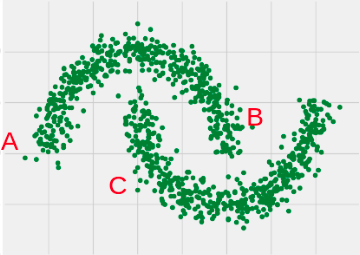
\includegraphics[width=0.8\textwidth]{images/two-moons.png}
\caption{
  In this picture, $A, B,$ and $C$ are data points in a two dimensional
    data set. Data-sensitive metrics have the property that the distance
    between $A$ and $B$ is short, while the distance between $A$ and $C$
    is long. 
 }
\label{fig:spec}
\end{figure}

  In this
  thesis, we explore how to efficiently compute two previously
  considered data-sensitive metrics: the edge-squared
  metric~\cite{vincent03}, and
  the nearest-neighbor metric~\cite{cohen15approximating}. Computing
  these metrics efficiently allows clustering to be performed on them in
  practice.

  The results we show on clustering are:
  \begin{enumerate}
  \item A $(1+\epsilon)$-spanner of the nearest neighbor metric, a notable example of a data sensitive
  distance, can be computed in nearly linear time in constant dimension.
  This will allow us to perform clustering using these metrics in a more
  efficient fashion than was previously known.
  \item The nearest neighbor metric and edge-squared metric are exactly
  identical in all cases.
  \end{enumerate}
  Prior to these results, it was not known how to compute either metric
  efficiently, and it was not even suspected that these two metrics were
  secretly identical. For this work, we make heavy use of the Kirszbraun theorem from
  metric embedding and computational geometry, also known as the Lipschitz extension theorem. We go into detail about these results in
  Chapter~\ref{sec:ds-main}.

  \section{Spectral Clustering in Large
    Datasets}\label{sec:spectral-limit}

  One of the most widely used clustering algorithms is known as
  spectral clustering~\cite{NgSpectral01}. We explore how it clusters data as the number of
  samples grows large. In this perspective, we make the assumption that
  the points are drawn from a probability density function. We show that
  spectral clustering has a key deficiency, and then devise a spectral
  clustering variant that addresses this deficiency. 

  \begin{enumerate}
  \item Given a large set of data drawn from a well-chosen and simple Lipschitz probability
  density, the most popular version of spectral clustering will converge
  to a bad cut of the data set, with unboundedly bad sparsity
  guarantees.
  \item Given a large data set drawn from any Lipschitz probability
  density, we present a new variant of spectral clustering that will
  converge to a cut of the data set with provable guarantees on
  the cut sparsity.
  \end{enumerate}
  
Traditional spectral clustering is one of the most robust and widely
used methods of clustering data. However, it has a major theoretical
issue. When a large number of points are drawn from a probability
density, then spectral clustering converges to something called a
\textbf{spectral sweep cut} of the underlying density.  However, this
spectral sweep cut can partition the probability density poorly, and
thus spectral clustering can converge to a poor partition of the data.

\begin{figure}[htbp]
\centering
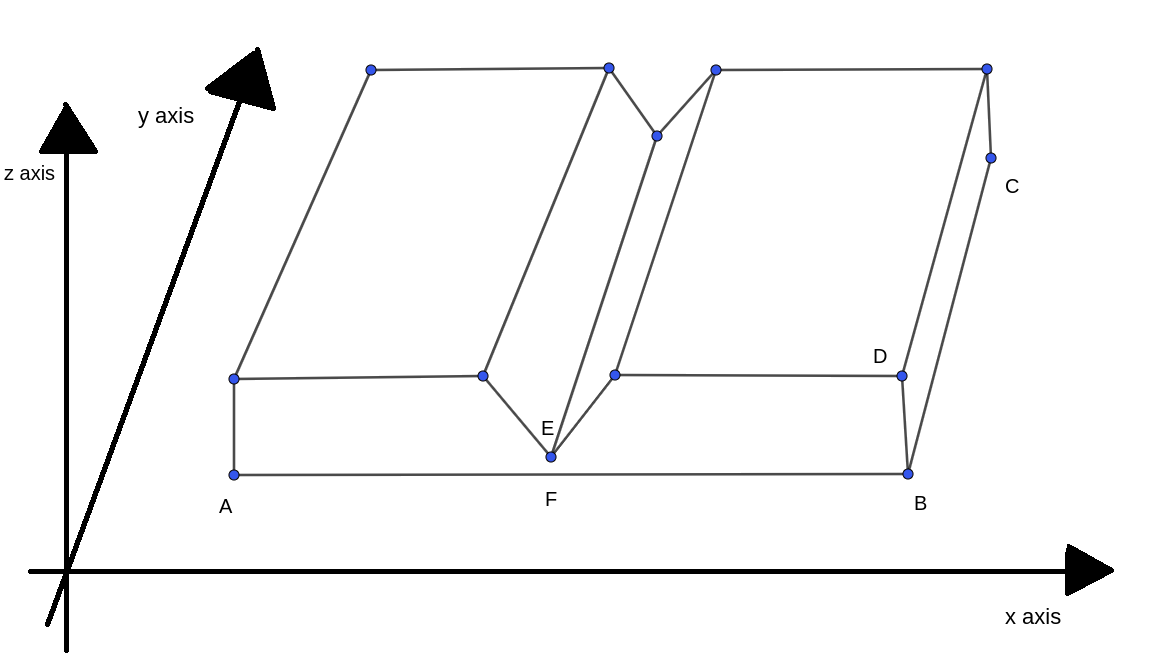
\includegraphics[width=0.6\textwidth]{images/counterexample.png}
\caption{
  We show a probability density function with support on the $xy$ plane,
  and value on the $z$ coordinate.  Traditional spectral clustering converges to a cut
  parallel to the $x$ axis, instead of the cut along the valley.
    In this figure,
  $BC$ is a constant
  factor longer than $AB$, and the height of the lowest point in the
  valley is
  $1/(BC)^{5/2}$. 
 }
\label{fig:spec}
\end{figure}

To remedy this, we build a new variant of the classical spectral
clustering method (splitting data into two clusters), and show that it
will, in the large data regime, generate a cut of the underlying probability
density with provable guarantees on the cut sparsity. At a high level,
this means that the generated cut cuts through low surface area while splitting the density into
two pieces of relatively high volume.

Spectral clustering itself is based on embedding data into new geometric
spaces, and thus the use of geometric embeddings features prominently in
our work. We will prove our variant of spectral clustering has good
sparsity guarantees through new extensions of the Cheeger and Buser
inequalities, applied to
probability densities. Cheeger and Buser inequalities are famous
inequalities traditionally used in the graph and manifold setting, with
the goal of relating fundamental eigenvalues with sparsest cut in each
of these settings. We will go into detail about spectral clustering in
Chapter~\ref{sec:spec-main}


\iffalse
\subsection{The Tool}
To prove that our spectral sweep cut variant has good isoperimetry
properties, we introduce Cheeger and Buser inequalities for Lipschitz
probability density functions. To do this, we create new definitions of
isoperimetry and eigenvalues in this setting. For past
definitions, one of the inequalities must fail. We apply our work to
give a new spectral algorithm for partitioning probability densities,
and discuss potential applications to spectral clustering.

Cheeger and Buser inequalities are the corner stone of spectral graph
theory, and have also been used widely to understand random processes on
Lipschitz manifolds. Our tool is to introduce these inequalities in the
probability density setting, which expands the range of objects on which
Cheeger and Buser inequalities apply.
\fi


\section{Spectral Graph Theory in Machine
  Learning}\label{sec:sgt}
  Graphs are often used in machine learning to encode the relationship
  between data points. There is a long history of applying graph theory
  algorithms on such graphs to perform machine learning primitives such
  as clustering, semi-supervised learning, and more.

  In Chapter~\ref{sec:sgt-main}, we develop spectral graph
  algorithms and complexity results on graphs arising from points in geometric space. Since
  data is often represented as points in geometric space, these
  results can be naturally applied to the above-mentioned machine
  learning questions. Our results can be used to speed up certain forms of spectral clustering, semi-supervised
  learning, and more.

  Results we will show on geometric spectral graph theory include: 
  \begin{enumerate}
  \item For certain complete geometric graphs arising from $n$ points in
  $d$ dimensions, we can compute a spectral
  sparsifier of the graph in $O(nd)$ time, where $n$ is the number of
  points and $d$ is the dimension.
  \item  For a large class of complete geometric graphs, it is
  impossible to solve the Laplacian to high accuracy in sub-quadratic
  time (assuming the Strong Exponential Time Hypothesis, or SETH).
  \end{enumerate}
  These results have applications to machine learning and physical
  simulations. In particular, the first algorithmic result will enable us to perform
  spectral clustering on these geometric graphs more efficiently, while
  the second result shows that the widely used fast-multipole method for
  computing forces between electrostatic charges in physics, has a
  run-time with unavoidable exponential dependence on dimension. We
  elaborate on these results in Chapter~\ref{sec:sgt-main}.
  

\iffalse
\section{Manhattan Kernels in Machine Learning, Metric Transforms, and Natural
  Language Processing}
      We develop a new tool, the representation theory of the real
      hyperrectangle, and prove new results in machine learning and algorithm design. Below, we describe our key application
      areas, and then overview what our new tool is and what it does.
\subsection{The Applications}
We describe our three main applications. 
\begin{enumerate}
\item First, we
give a classification of positive definite kernels with Manhattan
distance input. This is a Manhattan distance analog of a famous result
of Schoenberg that forms the foundations of modern kernel methods in
machine learning. 
\item Second, we categorize all functions which transform
Manhattan distances to Manhattan distances or squared Euclidean
distances. This is a Manhattan distance analog of a famous result by
Schoenberg on metric transforms, which is used in metric embedding
theory and has applications in harmonic analysis and sketching/embedding
of norms. 
\item Third, we prove that the only functions which always yield a low-rank matrix when applied entry-wise to a low-rank matrix are low-degree polynomials; this is a converse of a key idea behind the polynomial method in algorithm design and in the training of transformers in natural language processing. 
\end{enumerate}

In Section~\ref{rep} in our thesis, we go into detail about each of
these applications

\subsection{The Tool}
We introduced a new analytic technique we call
`representation theory of the real hyperrectangle'. At a high level,
  this technique gives simple expressions for computing the eigenvectors
  and eigenvalues of a large class of matrices which are defined in
  terms of hyperrectangles (high-dimensional analogues of rectangles).
  Later in my thesis, I will show that this class of matrices arises
  frequently in the study of linear algebraic tools for modern machine
  learning and algorithm design. As a result, we use our new technique
  to prove a number of new structural results in these areas.

  In Section~\ref{rep} in our thesis, we will explain what
  representation theory of the real hyperrectangle is, and why we name
  our tool that way. We will also show how this tool applies to each of
  the three main application areas.

\section{Patching a hole in spectral clustering}
We use Cheeger/Buser inequalities to patch a hole in spectral
clustering theory.
\subsection{The Application}
We put forward a new template for spectral clustering, which sidesteps
longstanding theoretical issues with traditional spectral clustering.

Traditional spectral clustering is one of the most robust and widely
used methods of clustering data. However, it has a major drawback. When a large number of points are drawn from a probability
density, then spectral clustering converges to something called a
\textbf{spectral sweep cut} of the underlying density.  However, this
spectral sweep cut can partition the probability density poorly, and
thus spectral clustering can converge to a poor partition of the data.

\begin{figure}[htbp]
\centering
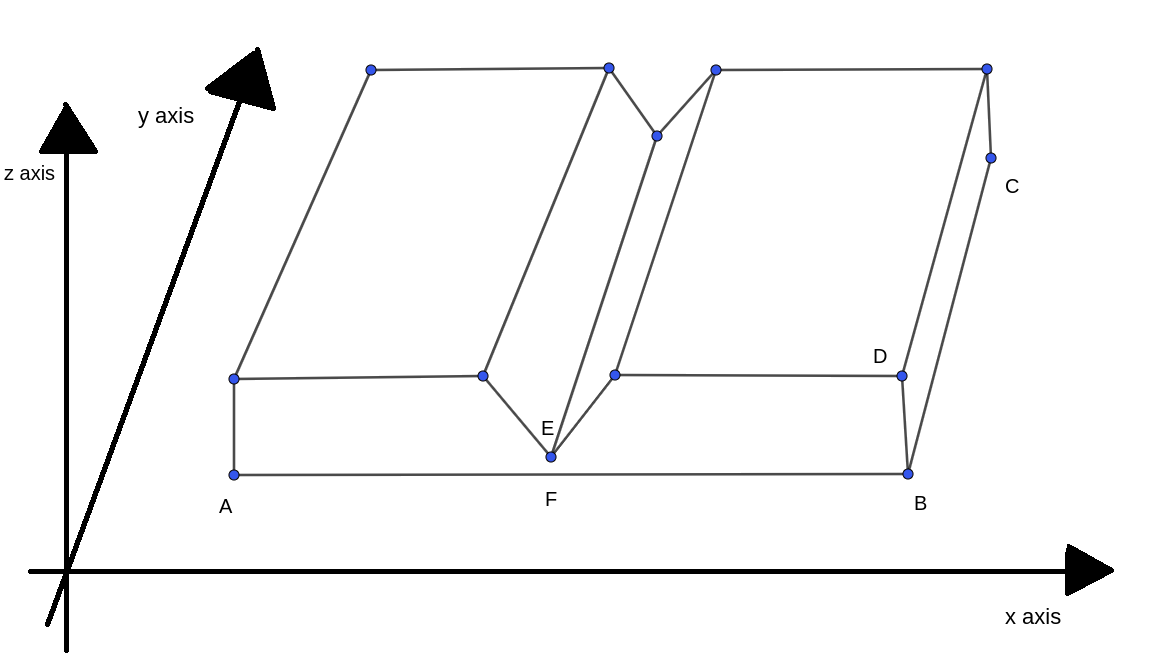
\includegraphics[width=0.6\textwidth]{images/counterexample.png}
\caption{
  We show a probability density function with support on the $xy$ plane,
  and value on the $z$ coordinate.  Traditional spectral clustering converges to a cut
  parallel to the $x$ axis, instead of the cut along the valley.
    In this figure,
  $BC$ is a constant
  factor longer than $AB$, and the height of the lowest point in the
  valley is
  $1/(BC)^{5/2}$. 
 }
\label{fig:spec}
\end{figure}

To remedy this, we build a new variant of the classical spectral sweep
cut, and show that it converges to a cut of the underlying probability
density with theoretical guarantees on the cut quality. We prove that
this new variant guarantees that the cut has good isoperimetry (for a
    modified definition of isoperimetry), which at a high level means
that it cuts through low surface area while splitting the density into
two pieces of relatively high volume.

We build this new spectral sweep variant in hopes that it will help
guide spectral clustering methods. There is a natural variant of
spectral clustering which we believe will converge to this variant of
spectral sweep cut, but we have not yet proven this convergence.

\subsection{The Tool}
To prove that our spectral sweep cut variant has good isoperimetry
properties, we introduce Cheeger and Buser inequalities for Lipschitz
probability density functions. To do this, we create new definitions of
isoperimetry and eigenvalues in this setting. For past
definitions, one of the inequalities must fail. We apply our work to
give a new spectral algorithm for partitioning probability densities,
and discuss potential applications to spectral clustering.

Cheeger and Buser inequalities are the corner stone of spectral graph
theory, and have also been used widely to understand random processes on
Lipschitz manifolds. Our tool is to introduce these inequalities in the
probability density setting, which expands the range of objects on which
Cheeger and Buser inequalities apply.

\section{Fast Multipole Method Hardness and Faster Spectral Clustering}
  We build hardness and algorithmic results for linear
  algebra tasks on a large suite of quadratically sized geometric
  graphs. Our tools pioneer geometric spectral algorithms. We apply our result to machine learning. 

\subsection{The Applications}
We use our results to gain insights about each of the following,
   seemingly unrelated tasks:

\vspace{1mm} \begin{tight_enumerate} \item \textbf{$n$-body simulation (one
    step)}: Given $n$ bodies $X$ located at points in $\mathbb{R}^d$,
  compute the gravitational force on each body induced by the other
  bodies.  \item \textbf{Spectral clustering}: Given $n$ points $X$ in
  $\mathbb{R}^d$, partition $X$ by building a graph $G$ on the points in
  $X$, computing the top $k$ eigenvectors of the Laplacian matrix $L_G$
  of $G$ for some $k\ge 1$ to embed $X$ into $\mathbb{R}^k$, and run
  $k$-means on the resulting points.  \item \textbf{Semi-supervised
    learning}: Given $n$ points $X$ in $\mathbb{R}^d$ and a function
    $g:X\rightarrow \mathbb{R}$ whose values on some of $X$ are known,
    extend $g$ to the rest of $X$.  \end{tight_enumerate}

\vspace{1mm}

Each of these tasks has seen much work throughout numerical analysis,
     theoretical computer science, and machine learning. The first task
     is a celebrated application of the fast multipole method of
     Greengard and Rokhlin~\cite{gr87, gr88, gr89}, voted one of the top
     ten algorithms of the twentieth century by the editors of
     \emph{Computing in Science and
       Engineering}~\cite{dongarra2000guest}.  The second task is
       \emph{spectral clustering} \cite{njw02, lwdh13}, a popular
       algorithm for clustering data. The third task is to label a full
       set of data given only a small set of partial
       labels~\cite{z05survey, csbz09, zl05}, which has seen increasing
       use in machine learning. One notable method for performing
       semi-supervised learning is the graph-based Laplacian regularizer
       method~\cite{lszlh19,zl05, bns06,z05}.

In our work, we show that the fast multipole method's exponential
dependence on dimension is necessary, and show hardness results for
semi-supervised learning using the graph-based Laplacian regularizer
method. We also show faster ways to perform spectral clustering for a
wide variety of geometric graphs $G$.
\section{Tools}
Our tools are primitives
spectral graph theory on a special class of dense graphs called
\emph{geometric graphs}, which can be used to gain new insights in each
for the above applications. 

For a function $\k:\mathbb{R}^d\times
\mathbb{R}^d\rightarrow \mathbb{R}$ and a set of points $X\subseteq
\mathbb{R}^d$, the \emph{$\k$-graph on $X$} is a graph with vertex set
$X$ and edges with weight $\k(u,v)$ for each pair $u,v\in X$. 

In our work, we initiate a theoretical study of the geometric graphs
for which efficient spectral graph theory is possible. In particular, we
attempt to determine for which (a) functions $\k$ and (b) dimensions $d$
there is a much faster, $n^{1+o(1)}$-time algorithm for each of (c)
  multiplication, sparsification, and Laplacian solving. 

Adjacency
matrix-vector multiplication, spectral sparsification, and Laplacian
system solving in geometric graphs are directly relevant to each of the
above problems, respectively:

\vspace{1mm} \begin{tight_enumerate} \item \textbf{$n$-body simulation (one
    step)}: For each $i\in \{1,2,\hdots,d\}$, make a weighted graph
$G_i$ on the points in $X$, in which the weight of the edge between the
points $u,v\in X$ in $G_i$ is $\k_i(u,v) := (\frac{G_{\text{grav}} \cdot
    m_u \cdot m_v}{\|u - v\|_2^2})(\frac{v_i - u_i}{\|u - v\|_2})$,
       where $G_{\text{grav}}$ is the gravitational constant and $m_x$
       is the mass of the point $x\in X$. Let $A_i$ denote the weighted
       adjacency matrix of $G_i$. Then $A_i\textbf{1}$ is the vector of
       $i$th coordinates of force vectors. In particular, gravitational
       force can be computed by doing $O(d)$ adjacency matrix-vector
       multiplications, where each adjacency matrix is that of the
       $\k_i$-graph on $X$ for some $i$.

\item \textbf{Spectral clustering}: Make a $\k$ graph $G$ on $X$. In
applications, $\k(u,v) = f(\|u-v\|_2^2)$, where $f$ is often chosen to
be $f(z) = e^{-z}$~\cite{l07,njw02}. Instead of directly running a
spectral clustering algorithm on $L_G$, one popular method is to
construct a sparse matrix $M$ approximating $L_G$ and run spectral
clustering on $M$ instead~\cite{chl16,csblc11, kmt12}. Standard
sparsification methods in the literature are heuristical, and include
the widely used Nystrom method which uniformly samples rows and columns
from the original matrix~\cite{cjkmm13}. 

If $H$ is a spectral sparsifier of $G$, it has been suggested that
spectral clustering with the top $k$ eigenvectors of $L_H$ performs just
as well in practice as spectral clustering with the top $k$ eigenvectors
of $L_G$~\cite{chl16}.  One justification is that since $H$ is a
spectral sparsifier of $G$, the eigenvalues of $L_H$ are at most a
constant factor larger than those of $L_G$, so cuts with similar
conductance guarantees are produced. Moreover, spectral clustering using
sparse matrices like $L_H$ is known to be faster than spectral
clustering on dense matrices like $L_G$ ~\cite{chl16, cjkmm13, kmt12}.

\item \textbf{Semi-supervised learning}: An important subroutine in
semi-supervised learning is completion based on
$\ell_2$-minimization~\cite{z05, z05survey, lszlh19}. Specifically,
  given values $g_v$ for $v\in Y$, where $Y$ is a subset of $X$, find
  the vector $g\in \mathbb{R}^n$ (variable over $X\setminus Y$) that
  minimizes $\sum_{u,v\in X,u\ne v} \k(u,v) (g_u - g_v)^2.$ The vector
  $g$ can be found by solving a Laplacian system on the $\k$-graph for
  $X$.  \end{tight_enumerate} \vspace{1mm}

In the first, second, and third tasks above, a small number of calls to
matrix-vector multiplication, spectral sparsification, and Laplacian
system solving, respectively, were made on geometric graphs. One could
solve these problems by first explicitly writing down the graph $G$ and
then using near-linear time algorithms \cite{ss11,ckmpprx14} to
multiply, sparsify, and solve systems. However, this requires a minimum
of $\Omega(n^2)$ time, as $G$ is a dense graph.

\section{Computing data-sensitive distances for clustering}
\subsection{The Applications}

\subsection{The Tool}

\section{Faster Effective Resistance Computation}
\subsection{The Applications}
\subsection{The Tool}
\section{Linear-time $2$-approximate deterministic principal eigenvalue computation on
    weighted lines}
\subsection{The Applications}
We present a deterministic algorithm for a linear-time, $2$-approximate
algorithm to compute the principal eigenvalue for the Laplacian of a generally weighted
line. 

  Fast computation of principal eigenvalues on graph Laplacians has been
  a longstanding goal of computer science. Traditional methods for this
  are randomized and involve logarithmic overhead. Algorithmic design
  has historically put high premium on linear-time algorithms and on
  deterministic algorithms. Our work is the first linear-time,
  deterministic algorithm for constant-approximating the eigenvalues of
  a weighted line. This is one of the simplest graphs for which the eigenvalues
  are not explicitly computable.
  
\subsection{The Tool}
  Hardy-Muckenhoupt inequalities $4$-approximates the fundamental eigenvalue of a graph with
  the quality of its so-called Hardy split. We will use this to give a
  dynamic programming algorithm for a
  deterministic, linear-time 4-approximation of the principal eigenvalue
  for the Laplacian of an arbitrarily weighted line.  We improve this to
  a $2$-approximation by creating a novel, tighter variant of the
  Hardy-Muckenhoupt inequality.  This Hardy-Muckenhoupt variant may be
  of independent interest.
\fi
